\documentclass[12pt]{article}
\usepackage[left=1in,right=1in,top=1in,bottom=1in]{geometry}
\usepackage{lmodern}
\usepackage{amsmath}
\usepackage{float}
\usepackage{graphicx}
\usepackage{enumitem}
\usepackage[font=footnotesize]{caption}
\usepackage{booktabs}
\setlist{noitemsep}
\begin{document}
\title{Appendix S\_ \\ Estimating Induced Mutation Rate}
\author{}
\date{}
\maketitle
\renewcommand\thefigure{A\arabic{figure}}
\section*{Nomenclature}
\par The parental generation (unmutagenized) is designated as $\mathrm{M}_{0}$.
Seed from the $\mathrm{M}_{0}$ is collected, and treated with radiation. The
seeds are then grown up into individuals, which are designated as the
$\mathrm{M}_{1}$ generation. Individuals in the $\mathrm{M}_{1}$ are then
carried by single-seed descent to the $\mathrm{M}_{2}$ generation. For brevity,
inbred lines derived from the initial mutagenesis event will be refered to as
$\mathrm{M}_{t+1}$, where $t$ refers to the number of generations of
single-seed descent since the mutagenesis event.

\par Similarly, for genetic transformation and tissue culture (GTTC) lines,
individuals are labeled as $\mathrm{T}_{t}$. However, in the case of GTTC,
the initial transformant is labeled as $\mathrm{T}_{0}$. Therefore, $t$ in the
case of GTTC refers to the number of generations since transformation, and not
1+generations, as in the case of mutagenesis.

\par A schematic showing the labeling of generations with relation to the
timing of mutagenesis or transformation is shown in the leftmost column of
Figure \ref{fig:fig1}.

\section*{Accounting for Spontaneous Mutations}
\begin{figure}[h]
    \centering
    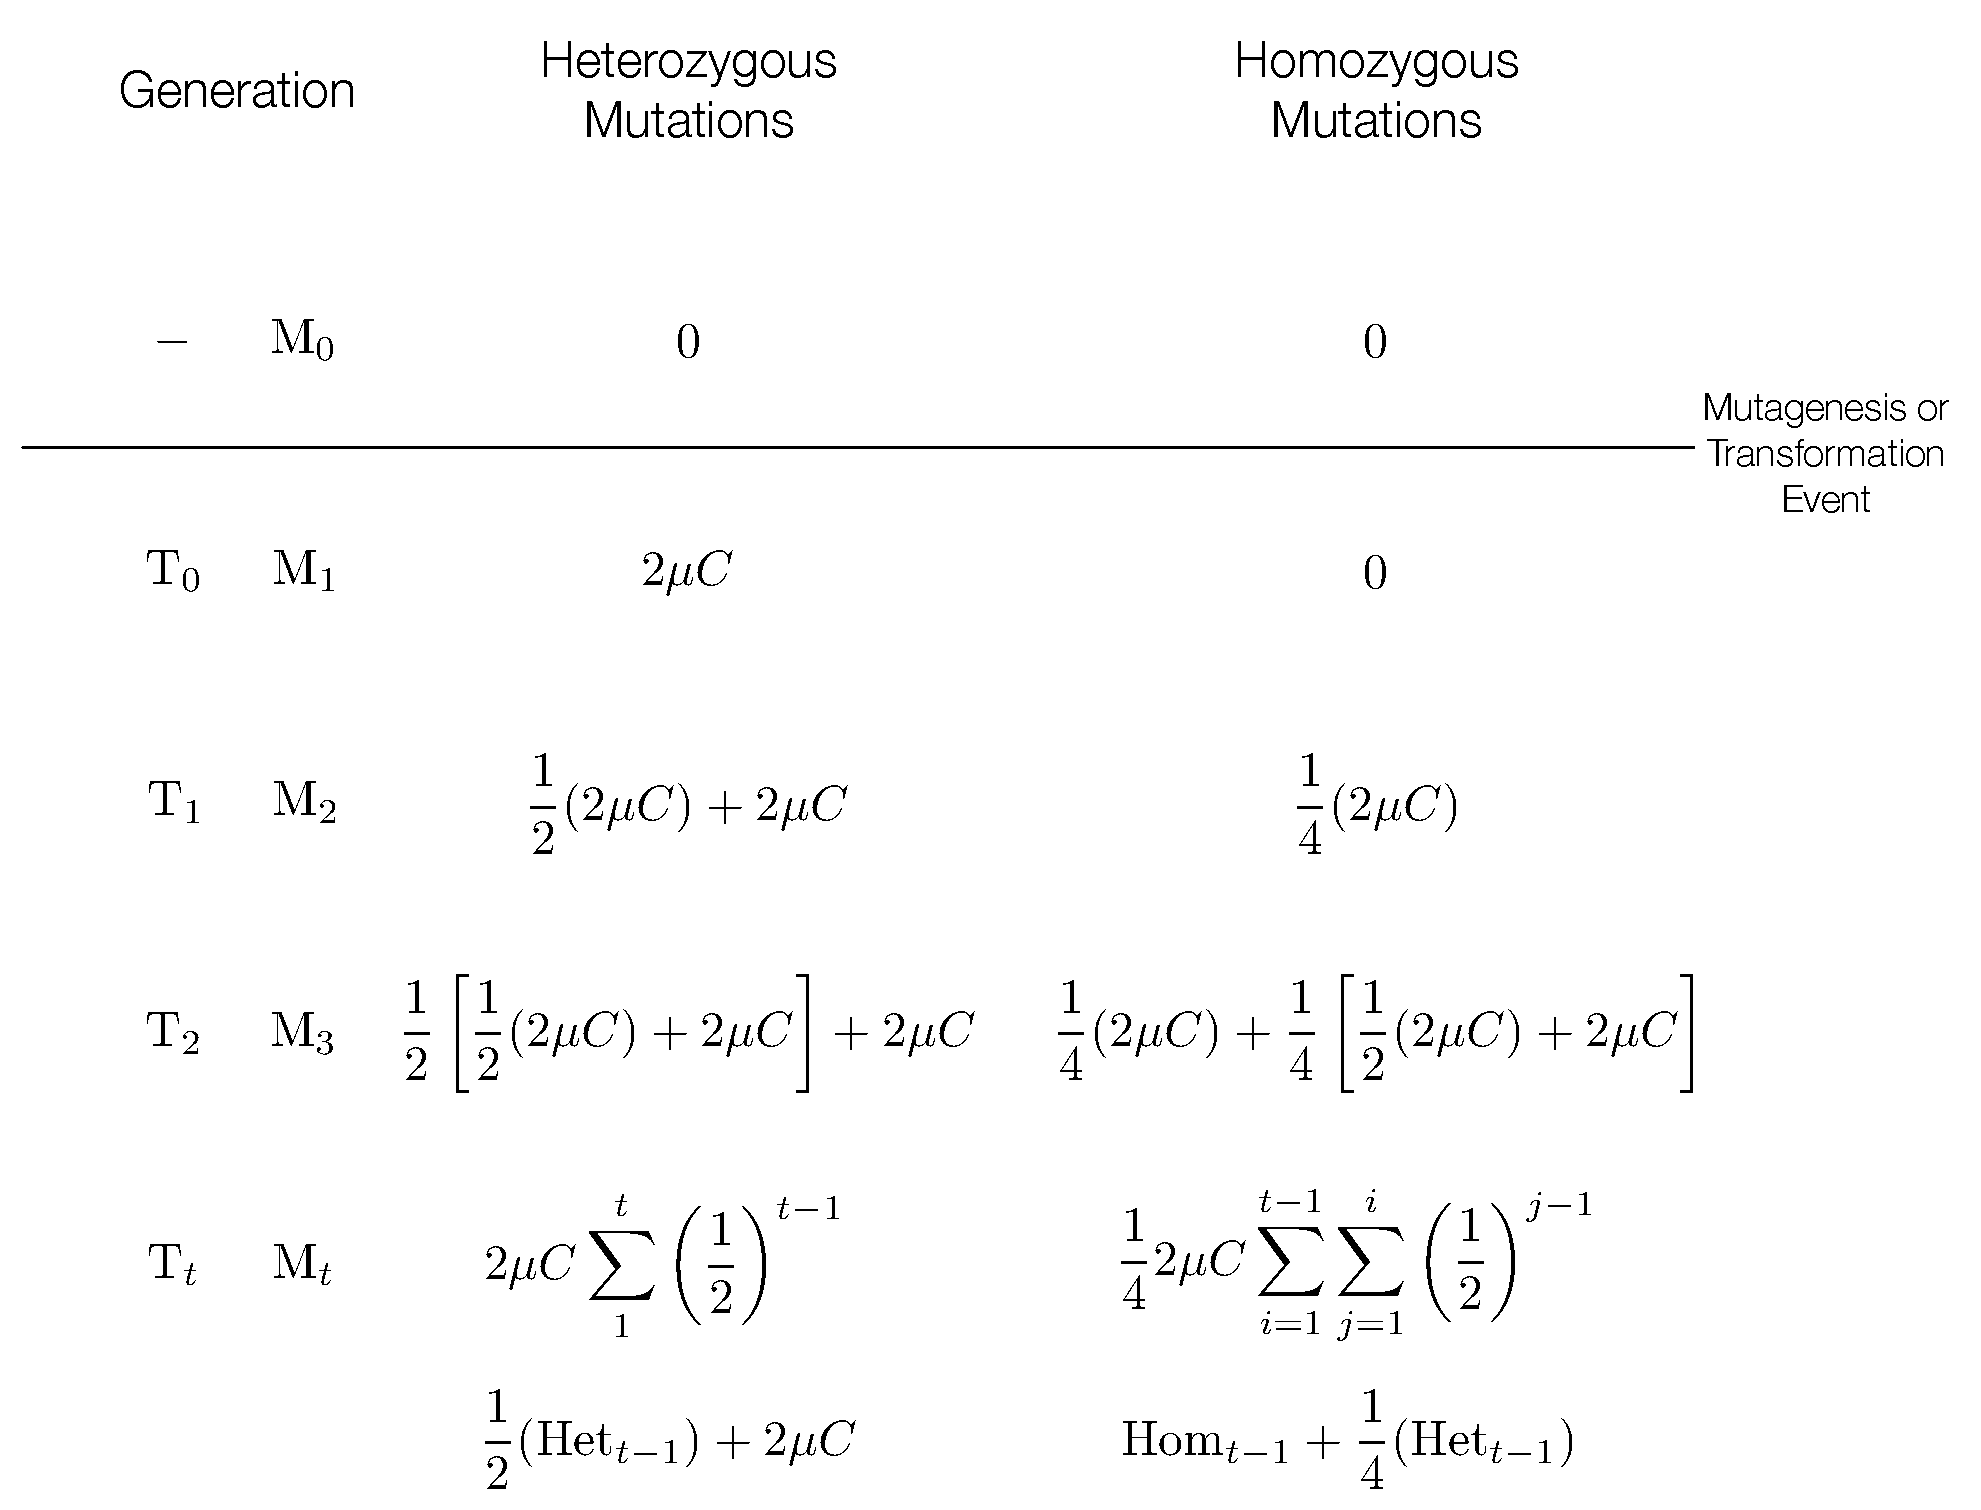
\includegraphics[width=0.7\textwidth]{Spontaneous_Mutations}
    \caption{The expected number of new spontaneous mutations in the
    heterozygous or homozygous states in the generations following mutagenesis
    or genetic transformation. New mutations arise in the heterozygous state at
    a rate of 2$\mu C ~\mathrm{bp}^{-1}\mathrm{gen}^{-1}$. One half of the
    heterozygous mutations remain heterozygous in the follow generation, and
    one quarter become homozygous. The last quarter are lost. See main text
    for assumptions and details.}
    \label{fig:fig1}
\end{figure}

\par To estimate the rate of induced mutation, we first need to estimate the
number of spontaneous mutations that would have accumulated over the course
of inbreeding. This is dependent on the per-base pair mutation rate, the size
of the genome, and the number of previously-accumulated mutations.

\par Figure \ref{fig:fig1} displays expectations for the number of mutations in
various generations that are derived from spontaneous mutations since the
mutatgenesis or transformation even. The expressions given rely on several
assumptions:
\begin{itemize}
    \item Back-mutation rate ($\nu$) is 0
    \item Each new mutation occurs at a different site (Infinite sites)
    \item Parental generation is homogenous and homozygous at every site
    \item Every site mutates with equal probability
    \item No linkage between sites
    \item New mutations are inherited with equal probability
\end{itemize}

\par Let new mutations arise at a rate $\mu$ per haploid site per generation in
a genome with $C$ haploid sites, and individuals reproduce by
self-fertilization. Under this scenario, the parental generation starts off
with 0 spontaneous mutations. The next generation is a product of one meiotic
event and thus undergoes one iteration of spontaneous mutation. All of the new
mutations that arise are heterozygous. The result is that the next generation
carries $2\mu C$ heterozygous mutations and 0 homozygous mutations. When the
next generation is produced, there will be not only self-fertilization, but
another iteration of spontaneous mutation. One half of the presently
heterzygous mutations will remain heterozygous, and one quarter will become
homozygous. Adding to the new mutations that arose, the next generation will
have $\frac{1}{2}(2\mu C) + 2\mu C$ heterozygous mutations, and
$\frac{1}{4}(2\mu C)$ homozygous mutations. Recusion expressions and summation
expressions are given in the final row of Figure \ref{fig:fig1}.
\par For estimating the number of specific mutational classes (\textit{e.g.,}
C:G mutations), it is necessary to adjust the mutation rate parameter ($\mu$)
and the genome size parameter ($C$) to reflect the mutational target.

\section*{Induced Mutation Rate}
\par To acheieve maximum confidence in variant calls, we focused only on
identifying homozygous variants in our sample (See main text methods).
However, when mutations enter the population (either spontaneously, or
through mutagenesis), they enter in the heterozygous stage. Because of this,
we need to back-calculate the inferred number of induced heterozygous mutations
from the number of observed homozygous mutations, some generations later. To do
this, we apply a scaling factor, since the number of observed homozygous
mutations is proportional to the number of induced heterozygous mutations.
Self-fertilization reduces the heterozygosity by half each generation. As
$t\rightarrow\infty$, the proportion of observed homozygous mutations will
approach $\frac{1}{2}$ of the induced heterozygous mutations, and this
represents an upper bound. Therefore, the scaling factor is 
$[\frac{1}{2} - (\frac{1}{2})^{t+1}]^{-1}$.

\par To estimate the rate of mutation induction, we used the observed number of
homozygous mutations in mutagenized lines, the number of generations they had
been maintained by single-seed descent, and the portion of the assayed genome
to estimate the number of induced heterozygous mutations. Let $S$ be the number
of observed homozygous variants in a line that has been maintained by $t$
generations of single-seed descent, and that $C$ haploid base pairs have been
assayed. Further, let $\mu$ be the haploid per-base pair per-generation rate of
spontaneous mutation. Then
$$
\dfrac
    {
        S -
        \dfrac{1}{4}
        2\mu
        C
        \sum_{i=1}^{t-1}
        \sum_{j=1}^{i}
        \left(
            \dfrac{1}{2}
        \right)^{j-1}
    }
    {
        C
        \left[
            \dfrac{1}{2} -
            \left(
                \dfrac{1}{2}
            \right)^{t+1}
        \right]
    }
$$
is the estimated rate of heterozygous mutation induction.

\section*{Numerical Estimates}
\par For estimating the number of spontaneous mutations in each generation, we
used estimates of $\mu$ from Ossowski \textit{et al.} 2010. Since the version
of the \textit{A. thaliana} reference assembly was not reported, we used genome
size and base content of the TAIR9 assembly (June 2009) to convert reported
per-genome mutation rates into per-base pair mutation rates. Our values for the
$C$ parameter were based on mapping of short-read sequencing data to the
\textit{Glycine max} V1 reference assembly (Schmutz \textit{et al.} 2010) and
applying alignment filtering critera. See the main text methods for details on
sequence data handling.

\par R scripts to perform the mutation rate estimation are available at
\textbf{[LINK]}.

\end{document}
